\appendix
\chapter{Appendix}

\section{CTM3 specifications}\label{app:CTM3}
\begin{table}[ht]
\centering
\begin{tabular}{|l|l|}
\hline
Value & PLAND-type   \\ \hline
0     & Ocean        \\ \hline
1     & Land         \\ \hline
2     & Lake         \\ \hline
3     & Small island \\ \hline
4     & Ice shelf    \\ \hline
\end{tabular}
\caption{\texttt{PLAND} is based on the \texttt{landsea.nc}-file from \protect\url{/work/projects/cicero/ctm_input/Indata_CTM3}}
\label{tab:PLAND}
\end{table}

\begin{figure}
    \centering
    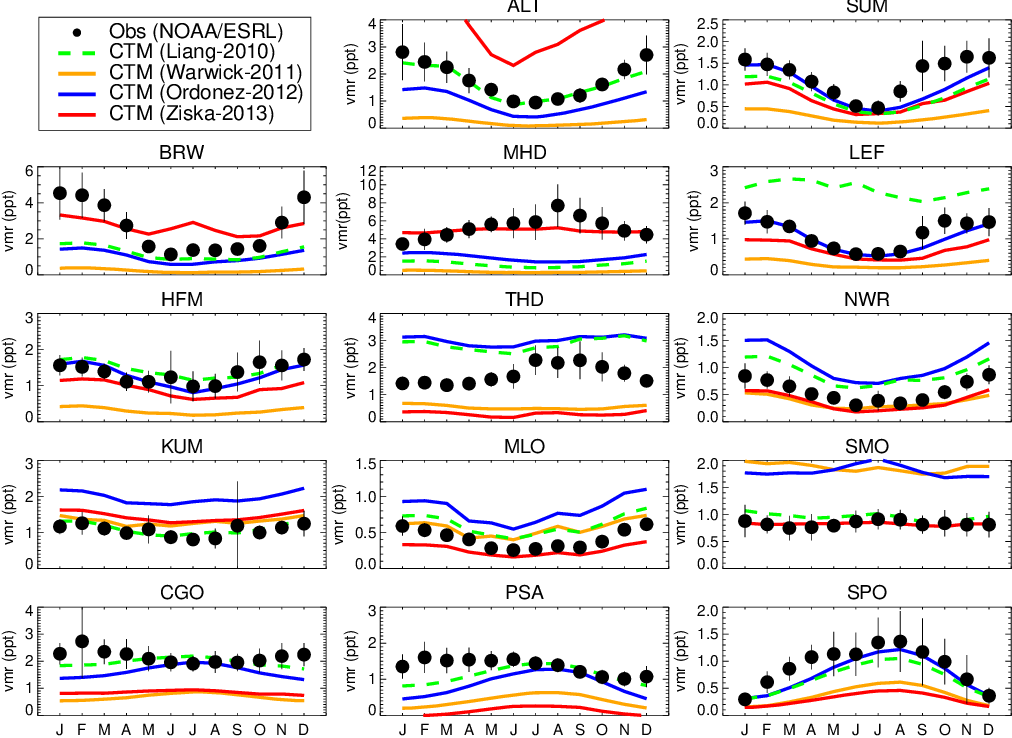
\includegraphics[width =0.7\linewidth]{Appendix/images/Hossaini2013_fig5_bromoform.png}
    \caption{Comparison of monthly mean mixing ratio (ppt) of $\chem{CHBr_3}$ output from \cite{Liang2010}, \cite{ziska}, warwick 2011, ordonez 2012}
    \label{fig:Hosaini_fig5}
\end{figure}

\begin{figure}
    \centering
    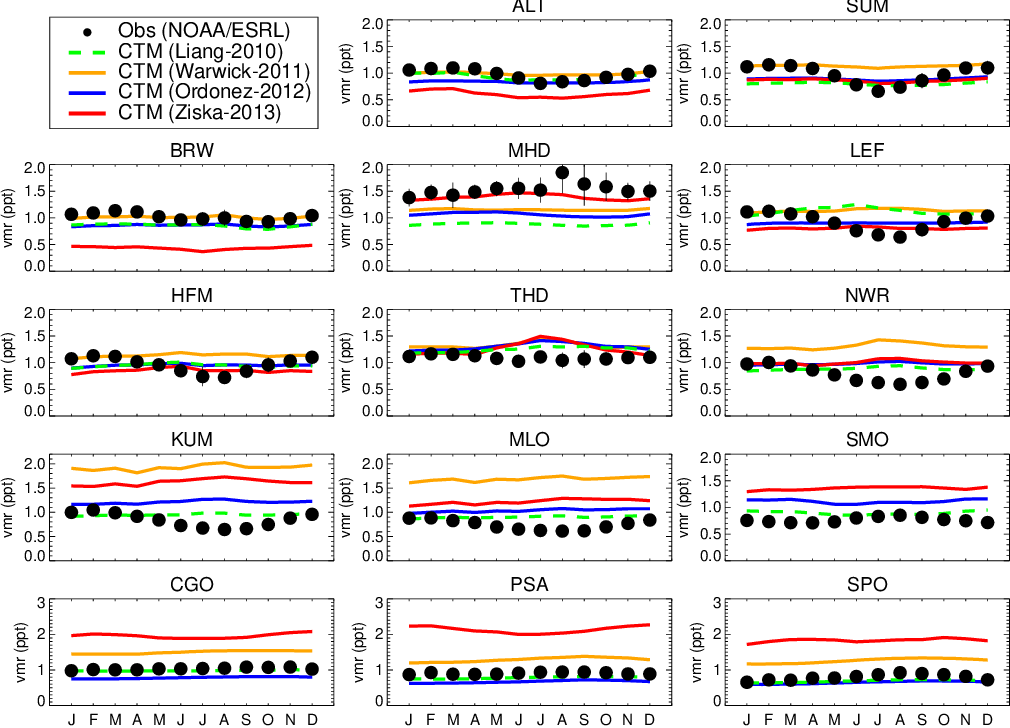
\includegraphics[width =0.9\linewidth]{Appendix/images/Hossaini2013_fig6_ch2br2.png}
    \caption{Comparison of monthly mean mixing ratio (ppt) of $\chem{CH_2Br_2}$ output from \cite{Liang2010}, \cite{ziska}, \cite{Warwick2006} and \cite{Ordonez2012}. The figure is adapted from \cite{Hossaini2013}}
    \label{fig:Hosaini_fig6}
\end{figure}



\cleardoublepage

\chapter{Chemical Unit Conversion}

The following appendix contains the conversion procedures concerning the CTM3 output as well as the conversion of station data to a mass mixing ratio. When analysing atmospheric data such as gases, it is most appropriate to use the mixing ratio (mol mol$^{-1}$), or mole fraction, as it is not dependent on pressure and temperature as the concentration (mol m$^{-3}$) is. It is defined as the ratio of the amount (or mass) of the substance in a given volume to the total amount (or mass) of all constituents in that volume (\cite{SeinfeldSpyros}). 

\medskip

The first section contains the formulas applied to the CTM3 data and the EBAS/NOAA data. The second section contains the \acrfull{cdo} procedure, which is a procedure for processing \acrshort{netcdf}-files. 

\section{Chemical Unit Conversion}

\subsection{Oslo CTM3}\label{sec:unit_conversion_CTM3}

The CTM3 data that are used are given in either monthly averages or tropospheric tracers (3-hour outputs). The monthly averages have units kg of species, and the 3-hour outputs have units g m$^{-3}$. 

\medskip

To obtain the mixing ratio from the monthly averages, the following was applied:

\begin{equation}
    \chem{X_{VMR}} = \frac{\chem{M_{air}}}{\chem{M_{X}}}\frac{\chem{X_{kg}}}{\chem{air_{kg}}}
    \label{eq:vmr_monthly_avg}
\end{equation}

In which $\chem{X_{VMR}}$ is the volume mixing ratio of the species, $\chem{M_X}$ and $\chem{M_{air}}$ are the molecular masses of the species of interest and air. $\chem{X_{kg}}$ and $\chem{air_{kg}}$ are the output data from CTM3 in kg of species. 

\medskip

In order to change the units of the tropospheric tracers (3-hour output), the following was performed: 

\begin{equation}
    \chem{X_{VMR}} = \frac{\chem{M_{air}}}{\chem{M_{X}}}\frac{\chem{X_{ g/cm^{3}}}}{\chem{\rho_{air}}}
    \label{eq:vmr_trop_tracer}
\end{equation}

In which  $\chem{X_{\mu g/m^{3}}}$ is the concentration of the species and $\chem{\rho_{air}}$ is the density of air (in $\mu g/m^{3}$). These are the output data from CTM3.


\subsection{EBAS/NOAA}\label{sec:unit_conversion_EBASNOAA}

The EBAS and NOAA data were provided in units $\mu g m^{-3}$, and were thus changes by: 

\begin{equation}
    \chem{X_{VMR}} = \frac{\chem{M_X}}{\chem{M_{air}}}\frac{\chem{X_{\mu g/cm^{3}}}}{\chem{\rho_{air}}}
\end{equation}

\section{Unit Conversion Using cdo}\label{sec:cdo}

The \acrshort{cdo}-software is a collection of operators for standard processing of climate and forecast data (\cite{cdo}). CDO is ideal for processing of large \acrshort{netcdf} datasets. 


\medskip

The \acrshort{cdo}-scripts were adapted from scripts provided by \cite{StefaniePersonal}. 

\begin{itemize}
    \item Load cdo by \texttt{module load cdo}
    \item \texttt{pwd} to the folder of interest
    \item \texttt{chmod +x "cdo file"} if there has been changes
    \item \texttt{./"cdo file" "Full path" --surface} (surface level is so far only possibility)
\end{itemize}

\cleardoublepage


\chapter{Figures}
%\addcontentsline{toc}{chapter}{Appendix B: Additional figures}
\cleardoublepage
